%----------------------------------------------------------------------------
\appendix
%----------------------------------------------------------------------------
\chapter*{Függelék}\addcontentsline{toc}{chapter}{Függelék}
\setcounter{chapter}{6}  % a fofejezet-szamlalo az angol ABC 6. betuje (F) lesz
\setcounter{equation}{0} % a fofejezet-szamlalo az angol ABC 6. betuje (F) lesz
\numberwithin{equation}{section}
\numberwithin{figure}{section}
\numberwithin{lstlisting}{section}
%\numberwithin{tabular}{section}

%----------------------------------------------------------------------------
\section{Az alkalmazás telepítése}
%----------------------------------------------------------------------------

Az alkalmazás telepítésének lépései következnek példáúl egy Ubuntu Linux rendszeren. Ha a rendszeren már van MongoDB és NodeJS akkor az első és második lépés kiugorható.

\begin{enumerate}
\item MongoDB adatbázis telepítése a \url{http://docs.mongodb.org/manual/tutorial/install-mongodb-on-ubuntu/} útmutató alapján:
\begin{enumerate}
\item \lstinline{sudo apt-key adv --keyserver hkp://keyserver.ubuntu.com:80 --recv 7F0CEB10}
\item \lstinline{echo 'deb http://downloads-distro.mongodb.org/repo/ubuntu-upstart dist 10gen' | sudo tee /etc/apt/sources.list.d/mongodb.list}
\item \lstinline{sudo apt-get update}
\item \lstinline{sudo apt-get install mongodb-10gen}
\item \lstinline{sudo service mongodb start}
\end{enumerate}

\item A NodeJs környezet telepítése: \lstinline{sudo apt-get install nodejs}
\item Az alkalmazás telepítése:
\begin{enumerate}
\item \lstinline{git clone git@github.com:chiller/mint.git}
\item \lstinline{cd mint/}
\item \lstinline{npm install}
\item \lstinline{node app.js}
\end{enumerate}
\item Az alkalmazás megnyitása böngészőben: \url{http://localhost:3000/}
\end{enumerate}

\clearpage\section{Az alkalmazás bemutatása}

Az alkalmazás publikusan elérhető \url{http://galacziendre-mint.jit.su/} címen. Google Chrome böngészőn működik a legnagyobb valószínűséggel.

\begin{figure}[!ht]
\centering
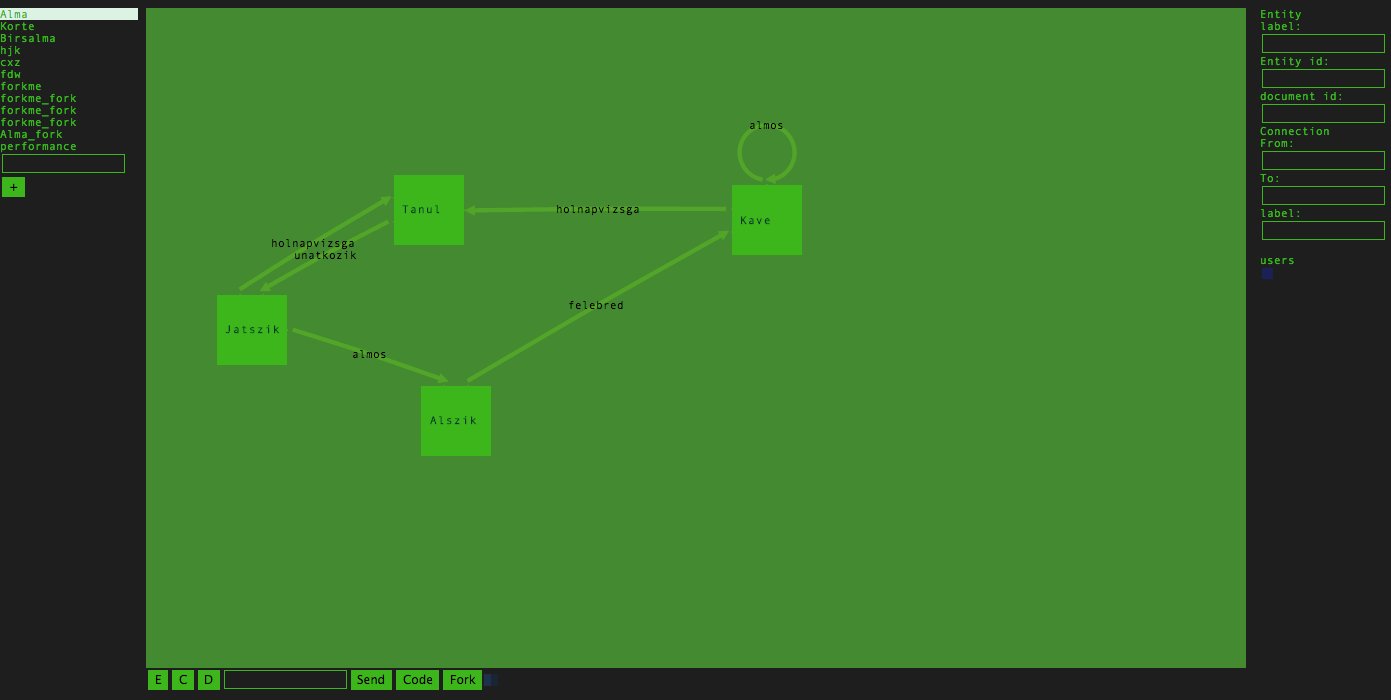
\includegraphics[width=160mm, keepaspectratio]{figures/demo.png}
\caption{A szerkesztő nézet} 
\end{figure}

A funkciók áttekintése:

\begin{enumerate}
\item A jobboldali panelben diagramok között választhatunk kattintással, ekkor betöltődik a kiválasztott diagram. Új diagram létrehozása a jobboldali panel beviteli mező és a + gomb megnyomása segítségével történik,
\item A baloldali panel a kiválasztott entitás, vagy a kiválasztott él tulajdonságait mutatja ezek közül a \lstinline{label} szerkeszthető, így lehet elem neveket szerkeszteni,

\item Az alsó panelben a ``Code'' gomb váltogat a diagram és a transzformációs kód nézet között, a ``Fork'' meg lemásolja a diagramot és megnyitja a másolatot.
\item A transzformációs nézetben a baloldali szövegdoboz várja az Underscore template kódot és a ``Compile gomb hatására'' a jobboldali szövegdobozba lefordul,
\item A diagramszerkesztőben E billentyűvel lehet létrehozni új elemet, egérrel lehet húzogatni az elemeket és élet úgy lehet húzni, hogy az elem helyett az elem címéből húzunk és akkor egy él húzódik, ezt egy másik elem címére kell húzni,
\item Elemek és élek kiválasztása kattintással történik. A törlésük backspace gombbal történik.
\end{enumerate}

%----------------------------------------------------------------------------
\clearpage\section{Az állapotgép kód generálása}
%----------------------------------------------------------------------------

\begin{figure}[!ht]
\centering
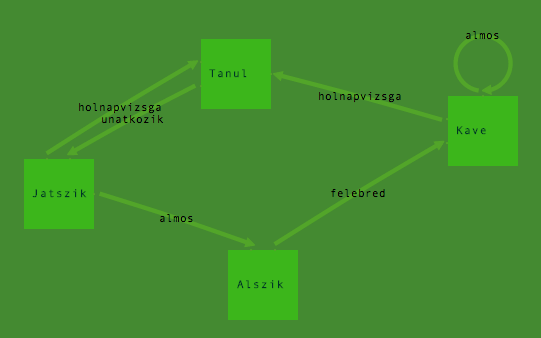
\includegraphics[width=100mm, keepaspectratio]{figures/tanulo.png}
\caption{A bemeneti diagram} 
\end{figure}


\begin{lstlisting}[caption=Az állapotgép kódgeneráló UnderscoreJS template-je]  

var sm = function() {

states = [

<% doc.entities.forEach(function(entity,i){
%>
  {"name": "<%= entity.title %>", 
   <%if(i==0){ %> "initial":true, <% }%>
  "events": {
    <% entity.connections_from.forEach(function(con){%>
        "<%=con.label%>":"<%=con.to%>",
    <%}) %>}
},<%
}) %>

]

 function StateMachine(states){
        this.states = states;
        this.indexes = {}; 
        for( var i = 0; i< this.states.length; i++){
            this.indexes[this.states[i].name] = i;
            if (this.states[i].initial){
                this.currentState = this.states[i];
            }
        }
        this.consumeEvent = function(e){
            if(this.currentState.events[e]){
                this.currentState = this.states[this.indexes[this.currentState.events[e]]] ;
                console.log(this.currentState.name);
            }
        }
        this.getStatus = function(){
            return this.currentState.name;
        }
    }
    return new StateMachine(states);
}

\clearpage

\end{lstlisting}



\begin{lstlisting}[caption=A generálás eredménye] 

var sm = function() {

states = [


  {"name": "Jatszik", 
    "initial":true, 
  "events": {"almos":"Alszik","holnapvizsga":"Tanul",}
},
  {"name": "Tanul", 
   
  "events": {"unatkozik":"Jatszik",}
},
  {"name": "Alszik", 
   
  "events": {"felebred":"Kave",}
},
  {"name": "Kave", 
   
  "events": {"holnapvizsga":"Tanul","almos":"Kave",}
},

]

 function StateMachine(states){
        this.states = states;
        this.indexes = {}; 
        for( var i = 0; i< this.states.length; i++){
            this.indexes[this.states[i].name] = i;
            if (this.states[i].initial){
                this.currentState = this.states[i];
            }
        }
        this.consumeEvent = function(e){
            if(this.currentState.events[e]){
                this.currentState = this.states[this.indexes[this.currentState.events[e]]] ;
                console.log(this.currentState.name);
            }
        }
        this.getStatus = function(){
            return this.currentState.name;
        }
    }
    return new StateMachine(states);
}

\end{lstlisting}
